\chapter{Base de datos: RethinkDB}
\label{chap:rethinkdb}

Mi sistema requiere guardar ciertos metadatos sobre las funciones en un sitio que perduren en el tiempo aunque el servidor se reinicie. He elegido RethinkDB como base de datos que me permita alcanzar ese objetivo.

RethinkDB\cite{rethinkdb} es una base de datos NoSQL pensada especialmente para notificar a tiempo real cambios en los datos y para gestionar de forma ultra sencilla las particiones y duplicidades por disponibilidad. Almacena y trabaja con documentos JSON enteros y es muy simple de usar y mantener.

\section{Documentos}

Almacena documentos JSON con toda su estructura en árbol. Esto simplifica la cantidad de tablas que necesitamos porque las relaciones uno a uno puede que tenga sentido eliminarlas en algunos casos y dejar los objetos inline; las relaciones uno a muchos se pueden guardar como una lista dentro del propio documento; y finalmente las relaciones muchos a muchos con propiedades adicionales en la relación se pueden guardar en uno de los dos lados y evitarnos la tabla intermedia que necesitaríamos en SQL. Ante todo estos trucos no son por reducir el número de tablas per se, aunque eso facilite las particiones y las duplicidades, sino por simplificar las estructuras de datos del programa dando lugar a un código de aplicación más sencillo y con menos errores.

Aparte de los tipos básicos de JSON como cadenas de texto, números, objectos y listas; RethinkDB define algunos tipos propios adicionales\cite{reqldatatypes} para cosas más avanzadas como fechas o geometría. Además los drivers de los diferentes lenguajes pueden elegir como leer y escribir esos valores de una forma más cómoda. Así por ejemplo el tipo de dato para fechas se puede leer como un \emph{Date} en Javascript, como un \emph{datetime.datetime} en Python o como un \emph{time.Time} en Go.

\section{Queries}

Las queries se realizan en un lenguaje propio denominado ReQL que se construye usando llamadas y métodos del lenguaje en el que estemos (Java, Python, etc.). Pueden comparar y actuar sobre cualquier propiedad del documento aunque esté anidada dentro de otra, se pueden filtrar listas, incluso se puede aplicar MapReduce\cite{mapreduce} sobre la tabla. A diferencia de otras bases de datos NoSQL RethinkDB si que permite hacer JOINs eficientes entre distintas tablas\cite{reqljoins}.

Todas las operaciones que definimos para hacer una query se transmiten a través de la red usando Protobuf donde el servidor C++ las ejecuta.

Ejemplo de query para filtrar una fila concreta:
\begin{minted}[baselinestretch=1.2]{js}
r.table('authors').filter(r.row('name').eq("William Adama"))
\end{minted}

Ejemplo de query con operaciones avanzadas como contar listas:
\begin{minted}[baselinestretch=1.2]{js}
r.table('authors').filter(r.row('posts').count().gt(2))
\end{minted}

\section{Dashboard}

Posee un dashboard integrado en la propia instalación que facilita la administración de los servidores. Como se aprecia en la figura \ref{fig:rethinkdb-dashboard} nada más llegar te da datos de rendimiento y carga de trabajo de los servidores. El problema que se ve en las capturas deriva de usar una instancia local con swap habilitado, algo indiferente para mi propósito de prototipo de sistema.

\begin{figure}[H]
    \centering
    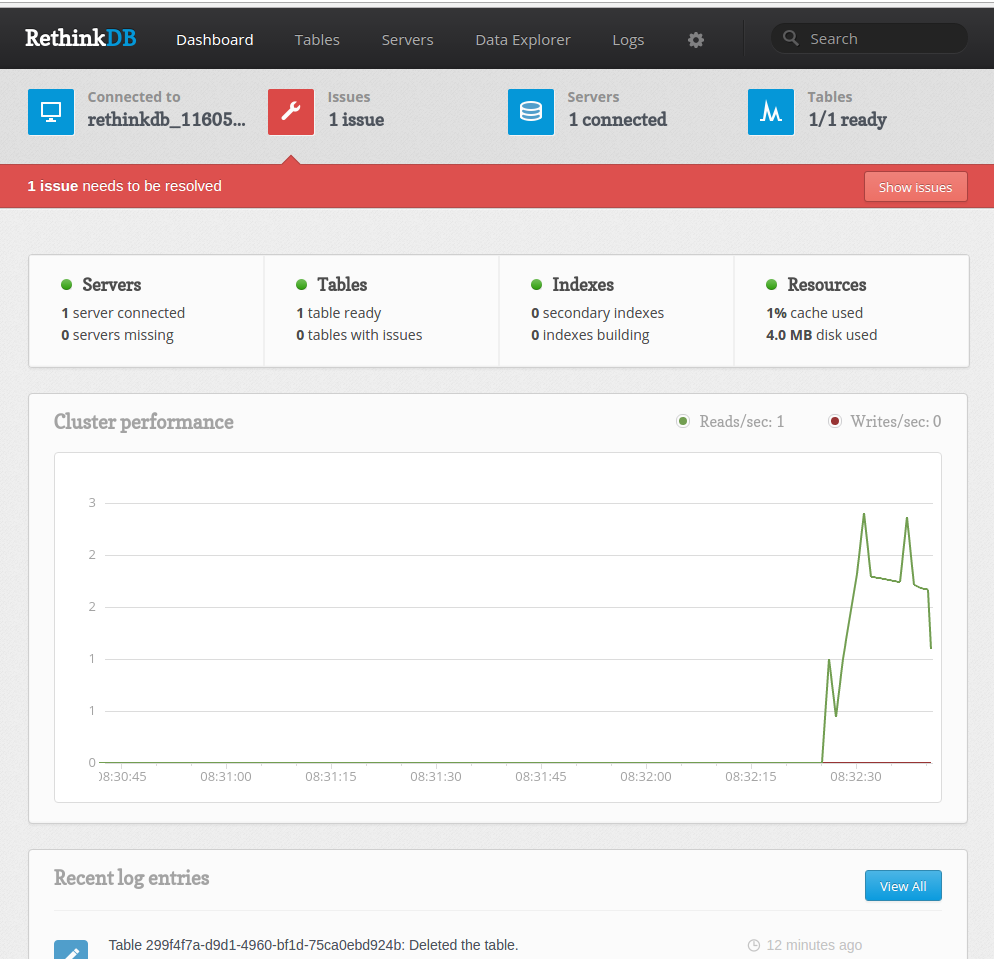
\includegraphics[width=\textwidth]{../images/rethinkdb/dashboard.png}
    \caption{RethinkDB Dashboard}
    \label{fig:rethinkdb-dashboard}
\end{figure}

Otro apartado del dashboard nos permite administrar las bases de datos, tablas y la repartición por servidores de los datos. Como se aprecia en la figura \ref{fig:rethinkdb-tables} es un panel muy simple con una funcionalidad clara.

\begin{figure}[H]
    \centering
    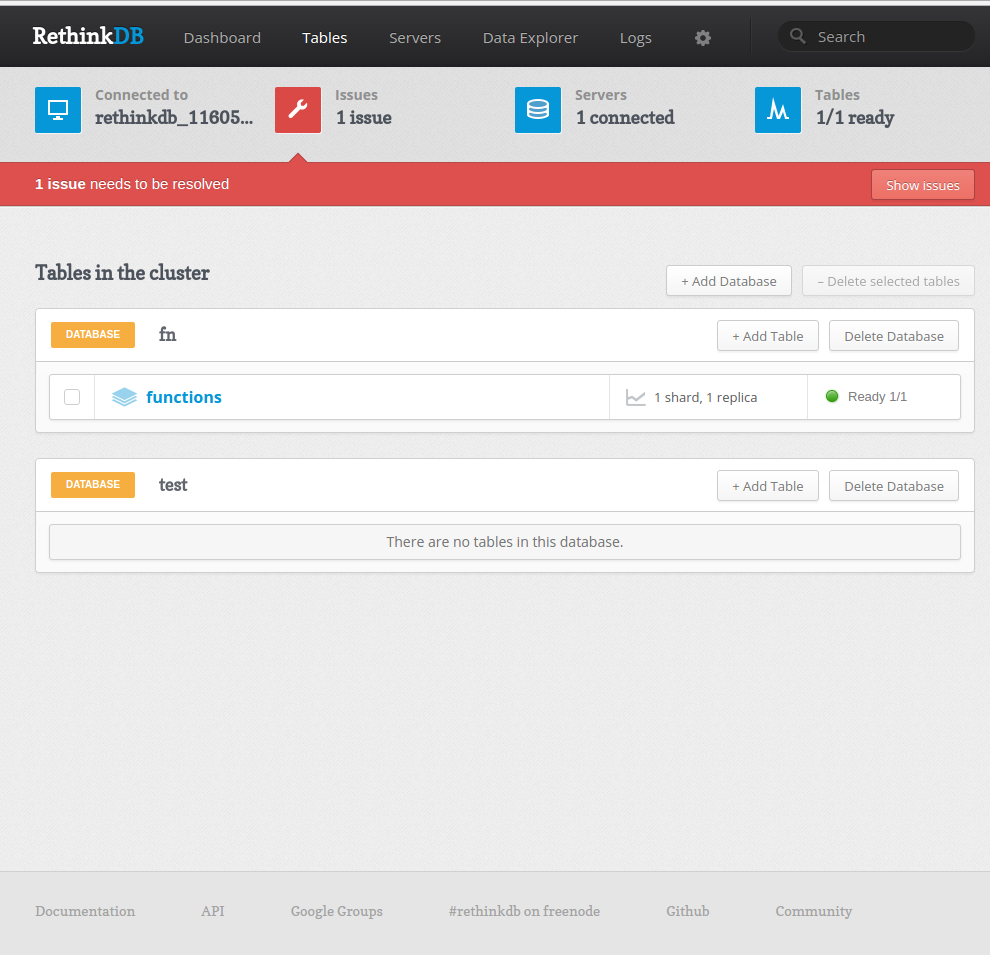
\includegraphics[width=\textwidth]{../images/rethinkdb/tables.png}
    \caption{Tablas RethinkDB}
    \label{fig:rethinkdb-tables}
\end{figure}

Finalmente el apartado más importante sea la consola de código. La base de datos lleva integrada un motor V8 para ejecutar Javascript. Desde el editor de la figura \ref{fig:rethinkdb-code} se pueden lanzar queries de consulta, lanzar tareas de administración como crear o eliminar tablas y cualquier otra cosa que se pudiera hacer desde una conexión normal desde código propio.

\begin{figure}[H]
    \centering
    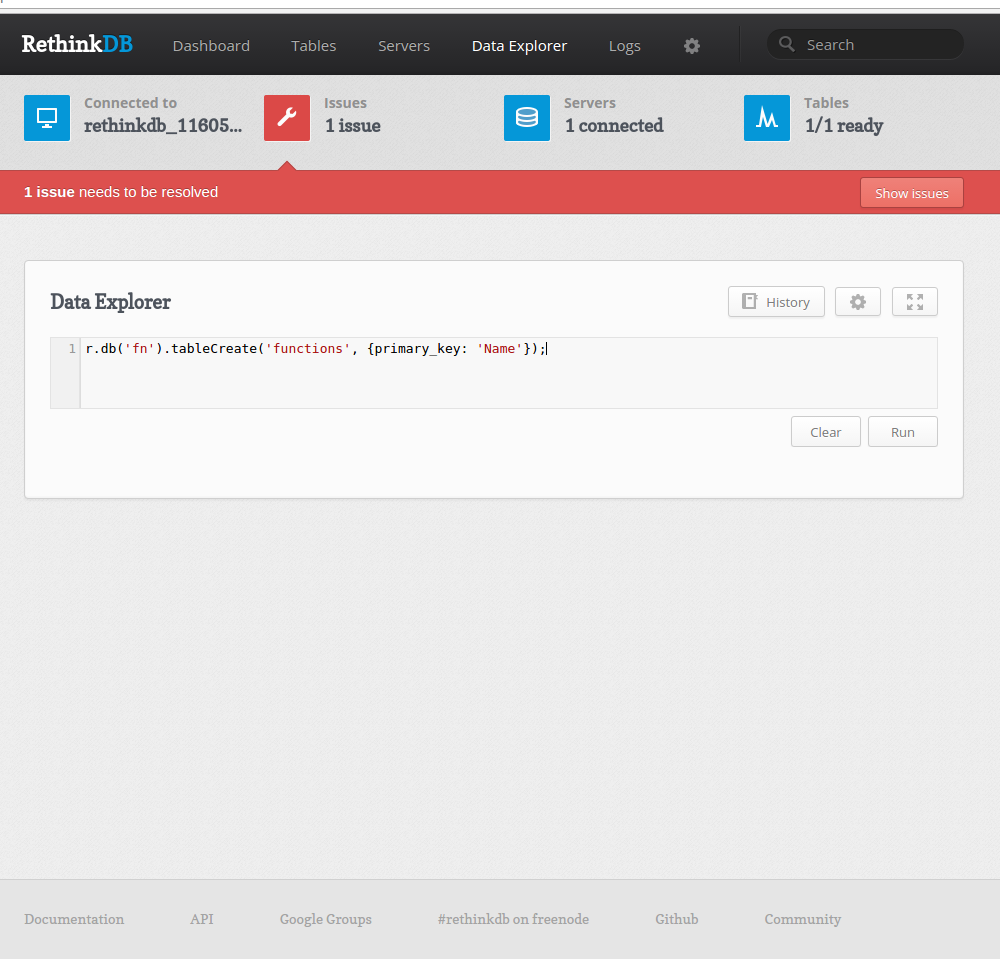
\includegraphics[width=\textwidth]{../images/rethinkdb/code.png}
    \caption{Consola de código de RethinkDB}
    \label{fig:rethinkdb-code}
\end{figure}

\section{Alternativas}
\label{sec:rethinkdb-alternativas}

Alternativas a cualquier base de datos hay muchas, más de las que se pueden referenciar y comparar en un solo documento. Voy a mencionar las típicas alternativas que se hubieran sugerido en una aplicación como la que yo he diseñado y porqué me he quedado finalmente con RethinkDB.

\subsection{MySQL}

Oracle MySQL es una base de datos relacional bastante conocida que modela los datos y sus relaciones mediante tablas simples.

No he usado MySQL porque quería la libertad de poder anidar datos para hacer más comodo el diseño de los modelos. Además las queries se hacen mediante SQL que el compilador de Go no puede validar ni comprobar; en cambio RethinkDB usa métodos de estructuras de la librería que si los usas incorrectamente pueden avisar del error mucho antes.

\subsection{MongoDB}

MongoDB es una base de datos no relacional bastante famosa que también es capaz de almacenar documentos JSON completos.

RethinkDB difiere en mejorar con respecto a MongoDB ciertos aspectos de bajo nivel\cite{redbvsmongo} con respecto a la durabilidad de los datos que la hace más robusta. Además los mecanismos de paralelización automática de queries en varios nodos son superiores. Ambas características son interesantes para producción cuando tienes que mantener el sistema durante mucho tiempo para un uso diverso. Lo que me convenció especialmente para el proyecto fué la interfaz administrativa tan cómoda y moderna que te permite desde hacer queries usando Javascript hasta controlar la replicación, disponibilidad y partición exacta de los datos en máquinas a un click de ratón.